When dealing with neurons, it must be kept in mind that there are several types of
neurons characterized by peculiar morphologies and arborizations, fundamental
to properly build an effective and reliable model.\\
To encode the structure of a neuron it is necessary to acquire images of the cell itself:
this is often done via radioactive or fluorescent markers, alternatively advanced optical
methods are often employed. Successively, the model has to be quantitatively characterized,
thus the dimensions of each cell element are measured.\\
Several softwares, such as \textit{NeuroMorpho}, were introduced to reconstruct 3D models of
neurons, allowing scientists to share them across the scientific community.

\subsection{Compartmental Models}
Generally, the morphology of the dendritic arborizations is the main attribute used to classify
neurons. Compartmental models are based on the idea that the various structures found in
a neuron can be modelled separately, then they are put together, constituting the
overall realistic and working model of the target cell.\\
In order to compartmentalize a neuron, the structure is divided into three main parts:
\begin{itemize}
    \item \textbf{Soma}: it is commonly approximated to a isopotential spheroid. the
          transition points between the soma and the dendritic tree are difficult to determine.
    \item \textbf{Dendritic Tree}: it is often modelled as a complex structure made by
          linked sequences of discrete cylinders, characterized by geometrical properties.
    \item  \textbf{Dendritic Spines}: they are the major target of synapses, making their
          modelling rather complex.
\end{itemize}
During the development of a model, it is crucial to keep in mind the following relatonships:
\begin{equation*}
    {Model\,fidelity}\propto{Amount\,of\,data}
    \hspace{2.5cm}
    {Simulation\,speed}\propto{\frac{1}{Model\,fidelity}}
\end{equation*}
An example of compartmental model is reported below, in particular the KCL and KVL for the
\(j-\)th element are shown:
\begin{figure}[H]
    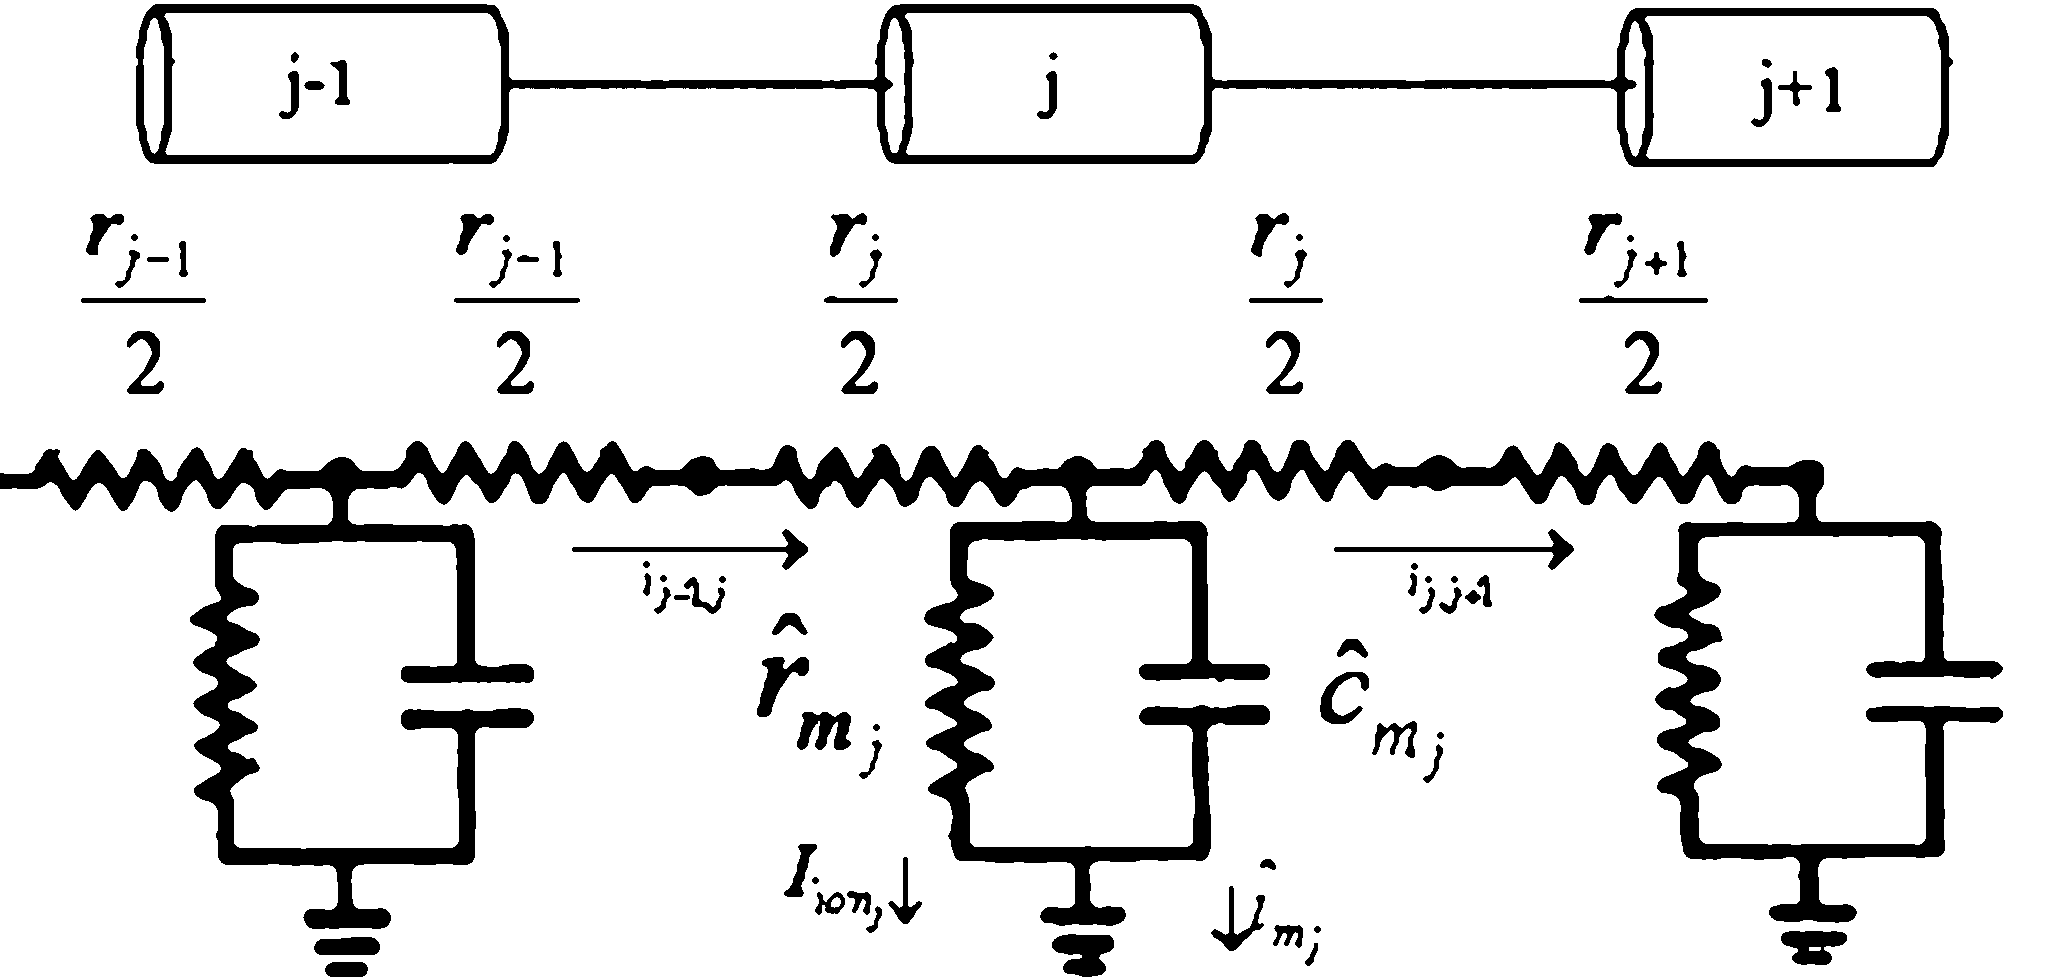
\includegraphics[scale=0.17]{03_1}
    \centering
\end{figure}
\begin{equation*}
    \begin{cases}
        \hat{i}_{m_{j}}=\hat{i}_{m_{j-1,j}}-\hat{i}_{m_{j}}=\hat{i}_{m_{j,j+1}} \\
        \hat{i}_{m_{j}}=I_{ion,j}+\hat{c}_{m}\frac{dV_{j}}{dt}+I_{stim,j}       \\
        \hat{i}_{m_{j}}=\frac{V_{j-1}-V_{j}}{r_{j-1,j}}-\frac{V_{j}-V{j+1}}{r_{j,j+1}}
    \end{cases}
    \Rightarrow
    \hat{c}_{m}\frac{dV_{j}}{dt}+I_{ion,j}+I_{stim,j}=g_{j-1,j}(V_{j-1}-V_{j})-g_{j,j+1}(V_{j}-V_{j+1})
\end{equation*}
In the equations above, \(r_{j}\) denotes the (specific) axoplasmatic resistance and \(I_{ion,j}\)
the ionic currents, including leakage and active channels, as well as synaptic contributions.
The main questions that should be answered when building a compartmental model regard the
compartmentalization criterion to employ, the estimation of the dendrites diameter if it is
not constant, and whether and how to take into account the dendritic spines. Therefore,
a segmentation (or compartmentalization) method is required.
\begin{figure}[H]
    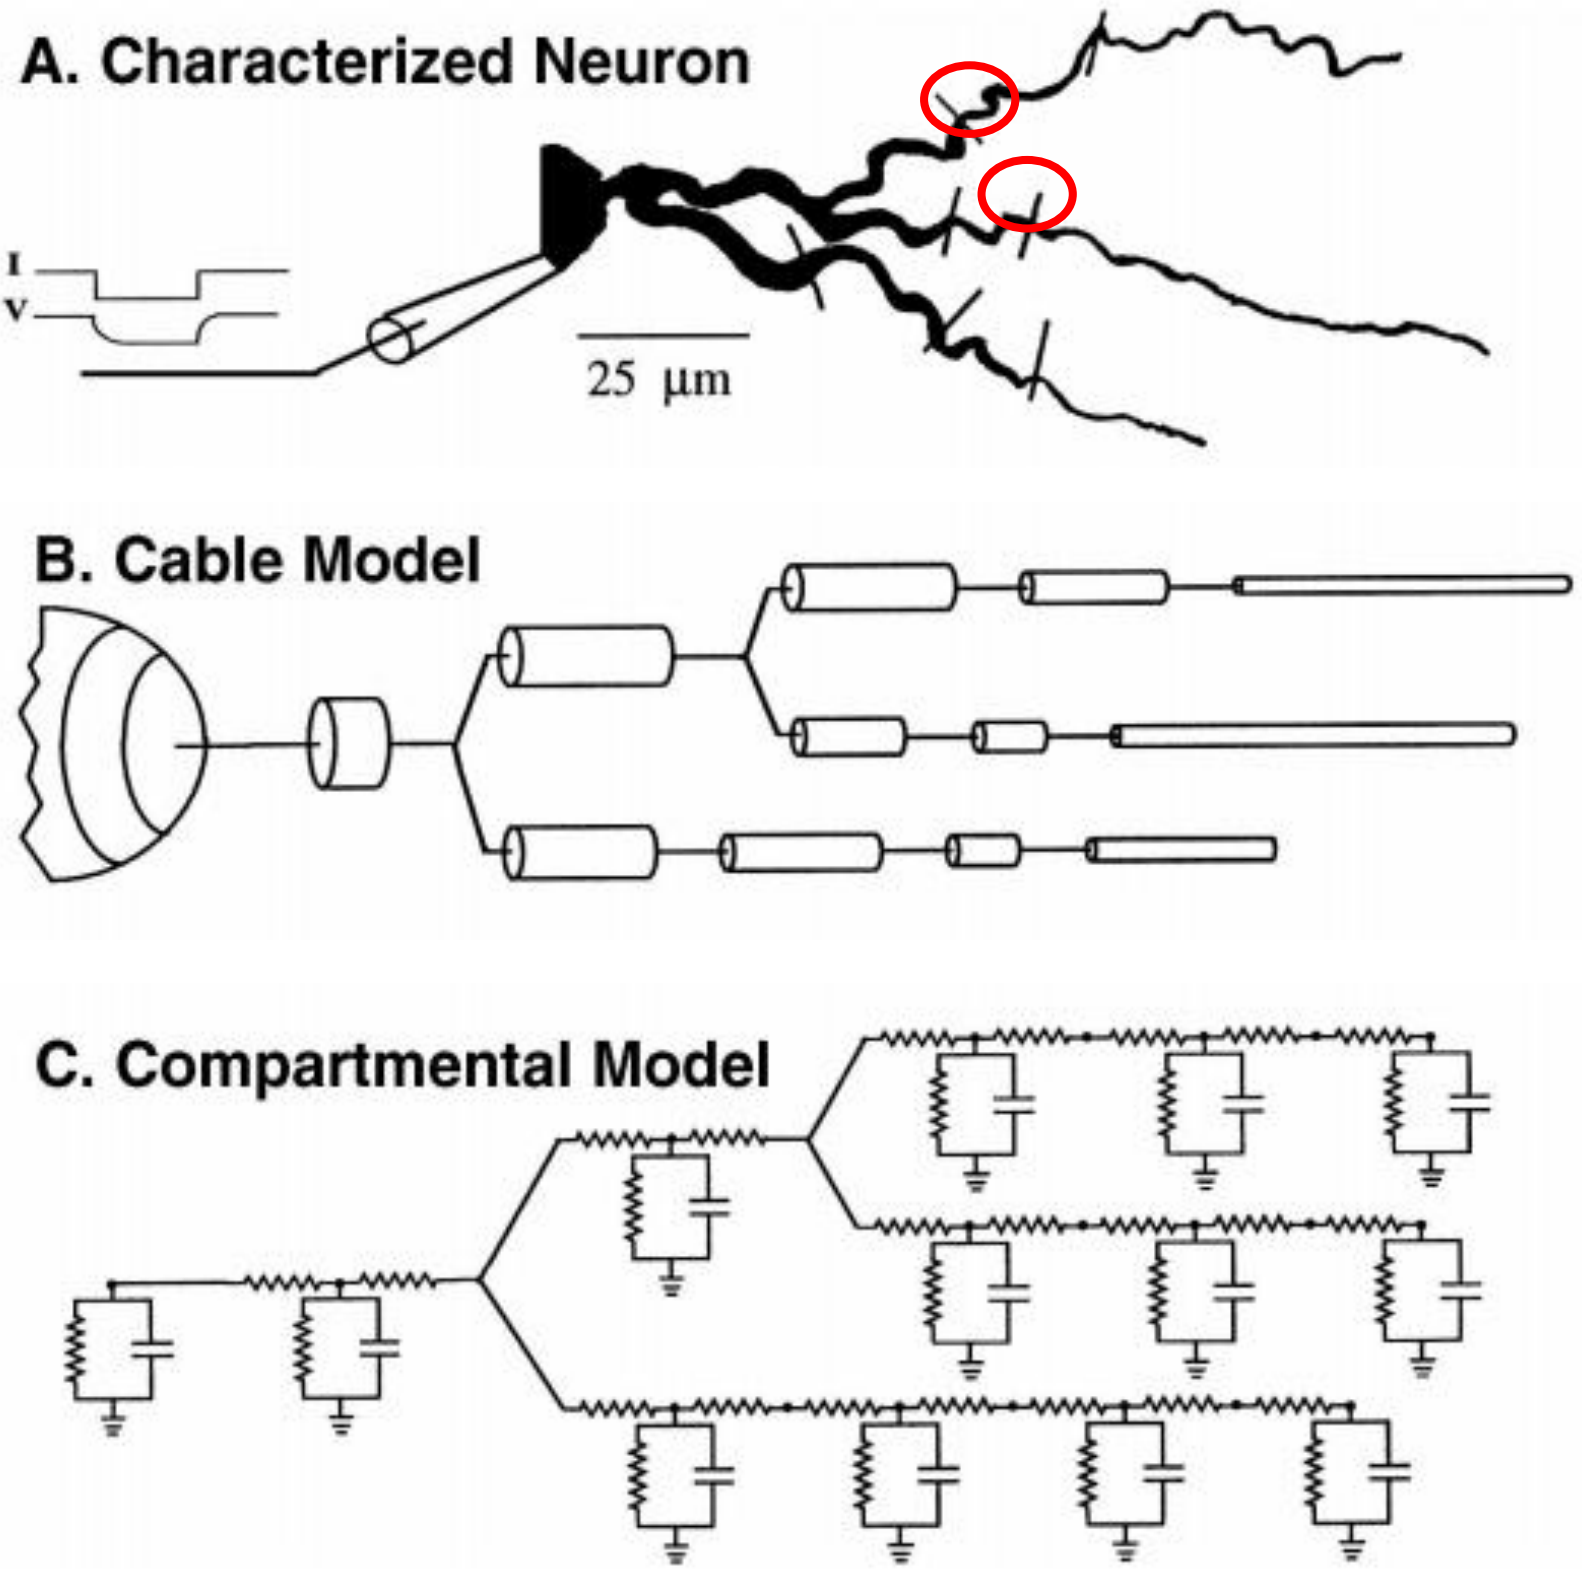
\includegraphics[scale=0.25]{03_2}
    \centering
\end{figure}
After characterizing the neuron from a geometrical point of view, a cable model, where
each dendritic segments is approximated to a cable with a specific diameter, is constructed.
Note that a threshold on the diameter is usually exploited, in order to have a discrete
set of diameters. Finally, each cable segment is considered to be isopotential and is modelled
through an equivalent electrical circuit.

\subsection{Complexity Reduction}
Given their nature, realistic and detailed compartmental models tend to be particularly
demanding from the computational point of view. Hence, the main idea is to simplify them,
losing some details in order to increase their efficiency. To do so, their level of
abstraction is increased.
\begin{figure}[H]
    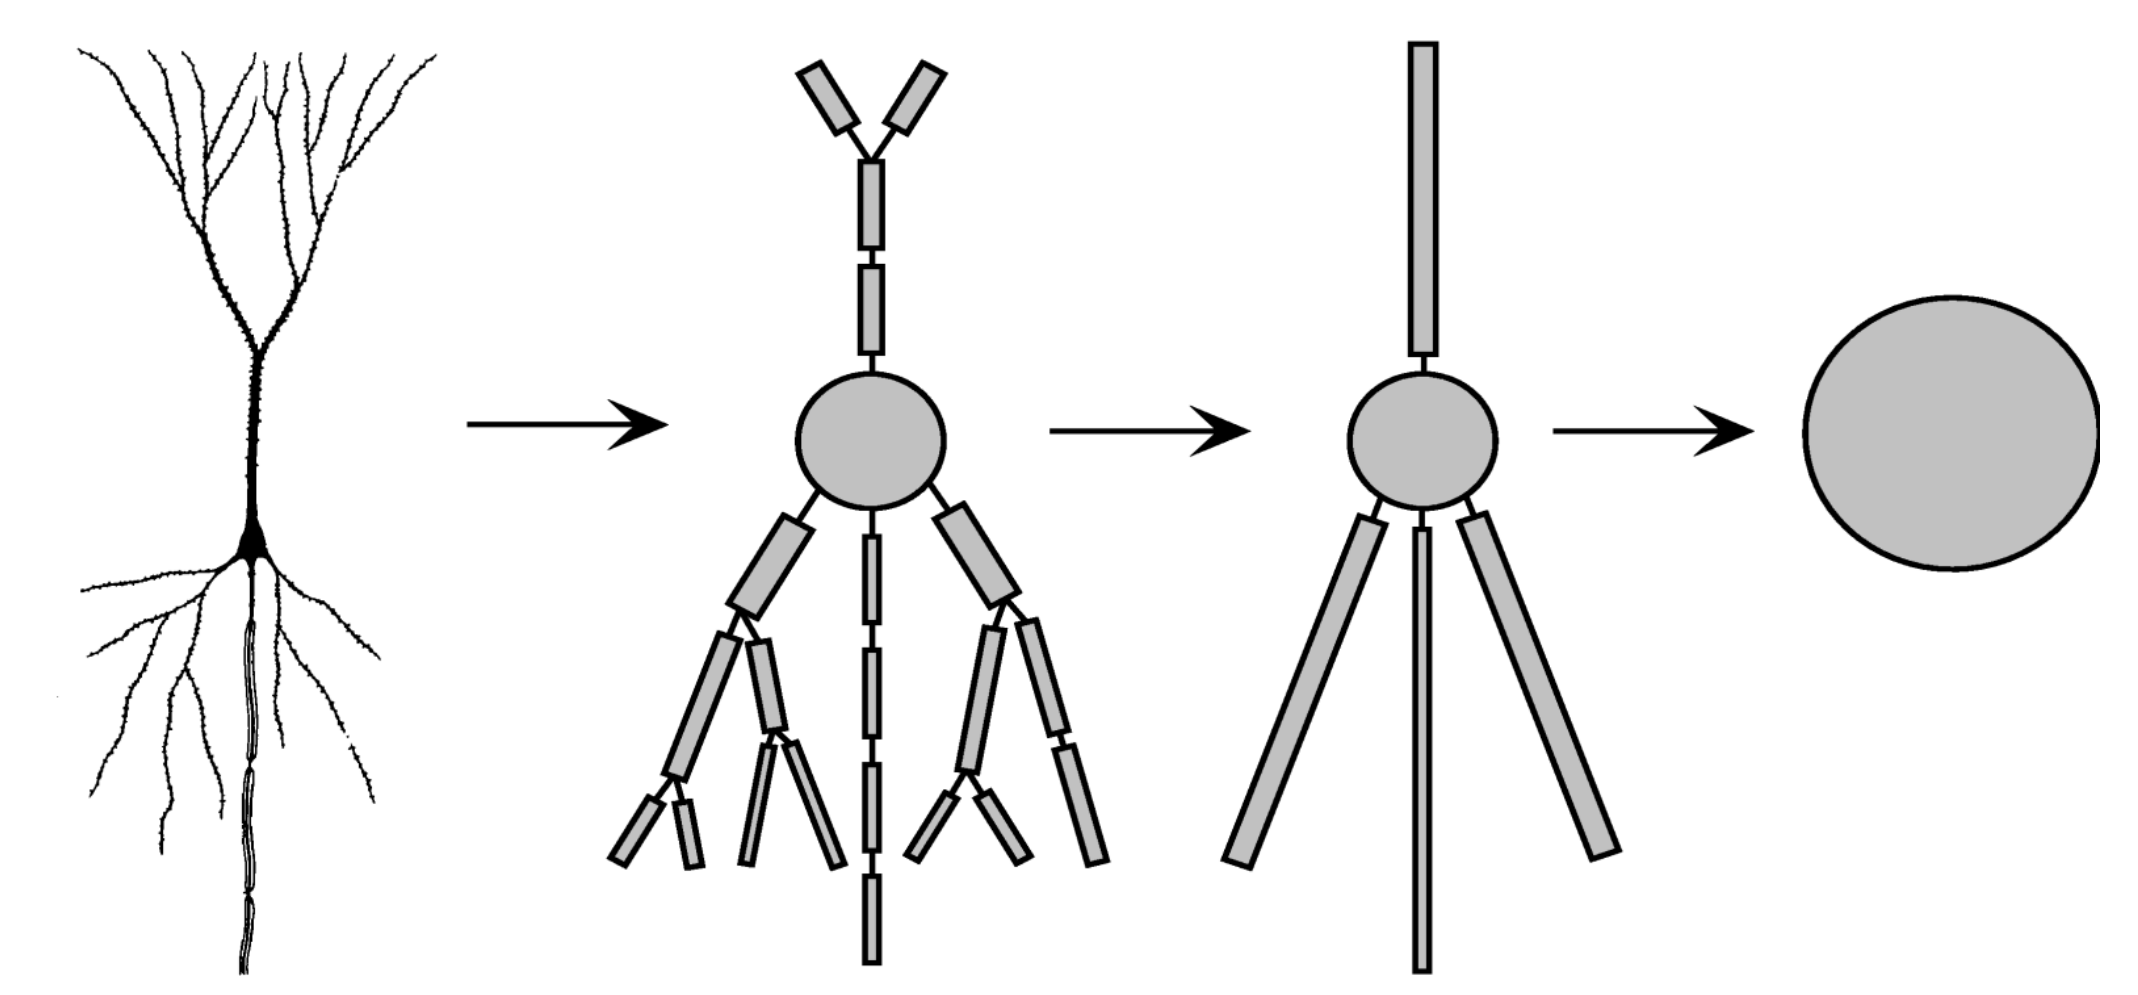
\includegraphics[scale=0.2]{03_3}
    \centering
\end{figure}
The aim is to reduce complexity while keeping the very same electrophysiological patterns,
such as bursts, spikes, and mixed activity. On the other hand, reducing a model inevitably
leads to losing certain features, ISI for instance, but it is not important as long as
these attributes are not relevant to characterize the considered model. The golden rule
when simplifying a neuronal model is that the input/output characteristic, which is
derived from stimulations, should not change. Note that the neuron spontaneous activity is
instead strictly related to the cell morphology, thus it is extremely difficult to
preserve it during model reduction.
\begin{figure}[H]
    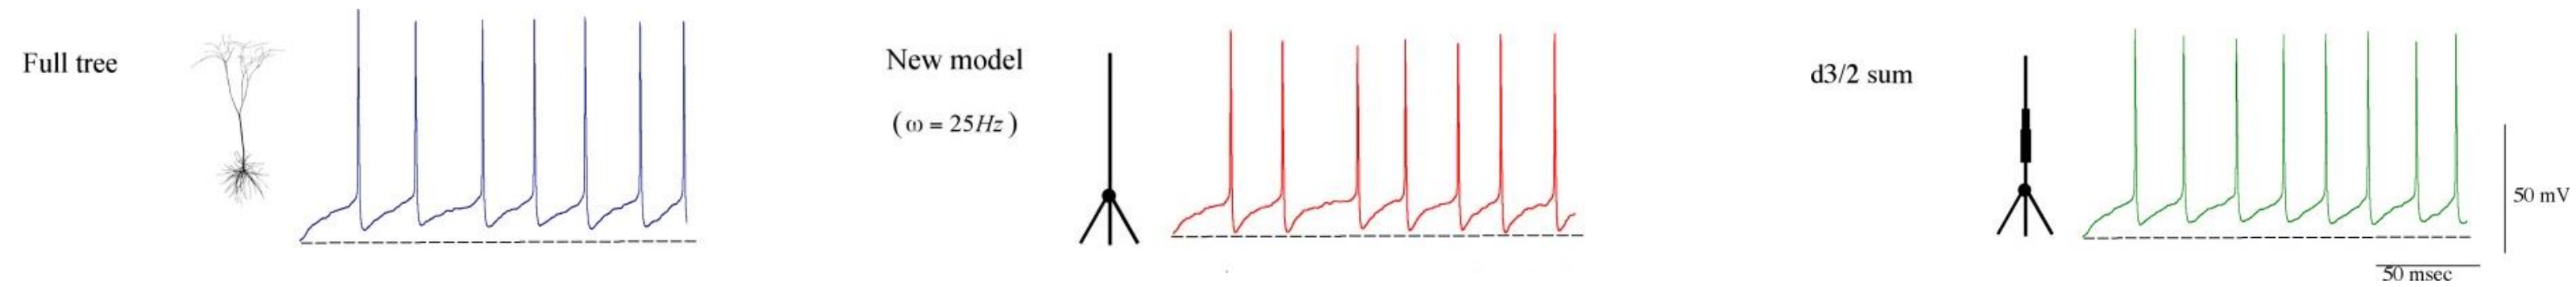
\includegraphics[scale=0.25]{03_4}
    \centering
\end{figure}
\paragraph{The Rall's Equivalent Cylinder}
The main idea is that the whole dendritic tree of a neuron can be represented as a single cylinder
having a constant diameter. In the model proposed by Rall, the soma is substituted by
a compact region (a single compartment), while the entire dendritic tree is replaced by
a single equivalent cylindrical cable. Said so, it is crucial to properly select the
geometrical and electrical properties of such a cylinder, such as its radius \(a\) and
length \(L\).
\begin{figure}[H]
    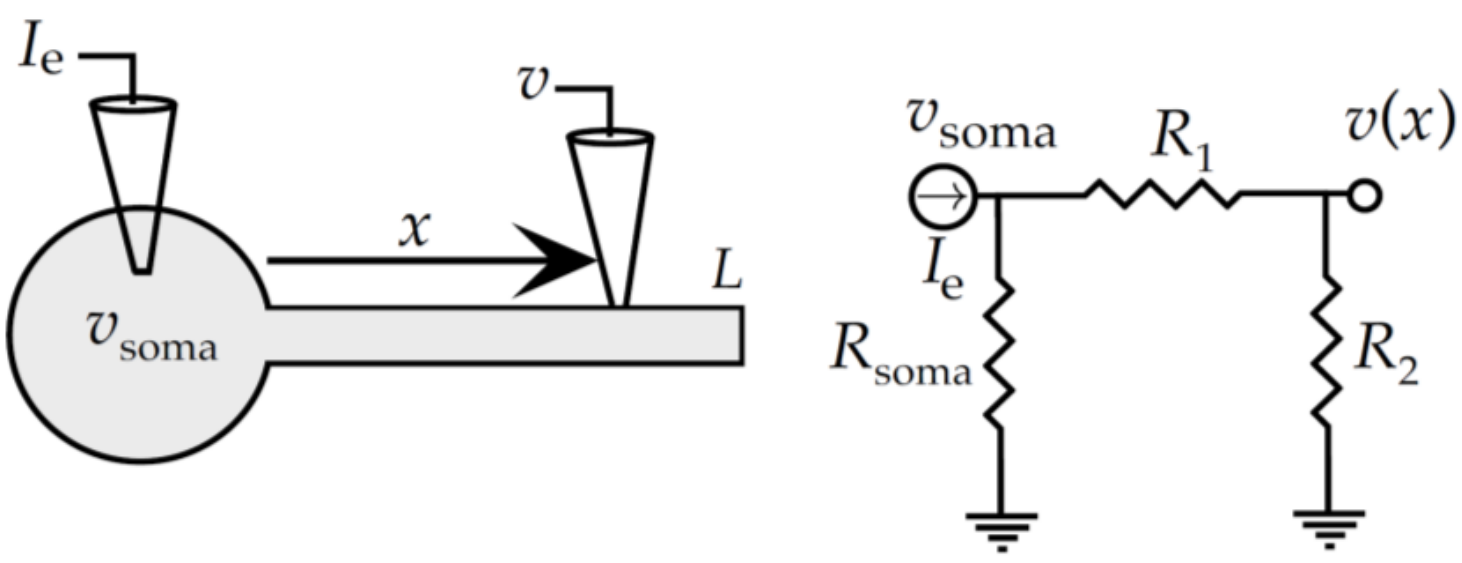
\includegraphics[scale=0.35]{03_5}
    \centering
\end{figure}
\(L\) and \(a\) are carefully selected to match two critical properties of the dendritic
tree. As a matter of fact, \(L\) is related to the average electrotonic length,
determining the degree of attenuation of the electrical input as a function of the distance.
The electrotonic length is measured by summing all the electrotonic segment lengths according
to the designated end point and then computing an average measure, describing the average
signal decay rate between the input and the output ends.\\
Differently, \(a\) is employed in the computation of the total surface area \(2\pi{a}\cdot{L}\),
crucial to correctly model the membrane resistance and capacitance of the neuron. The Rall's
model neuron input resistance \(R_{in}\) can be derived as follow:
\begin{equation*}
    R_{in}=\frac{(R_{1}+R_{2})R_{soma}}{(R_{1}+R_{2}+R_{soma})}
\end{equation*}
\begin{figure}[H]
    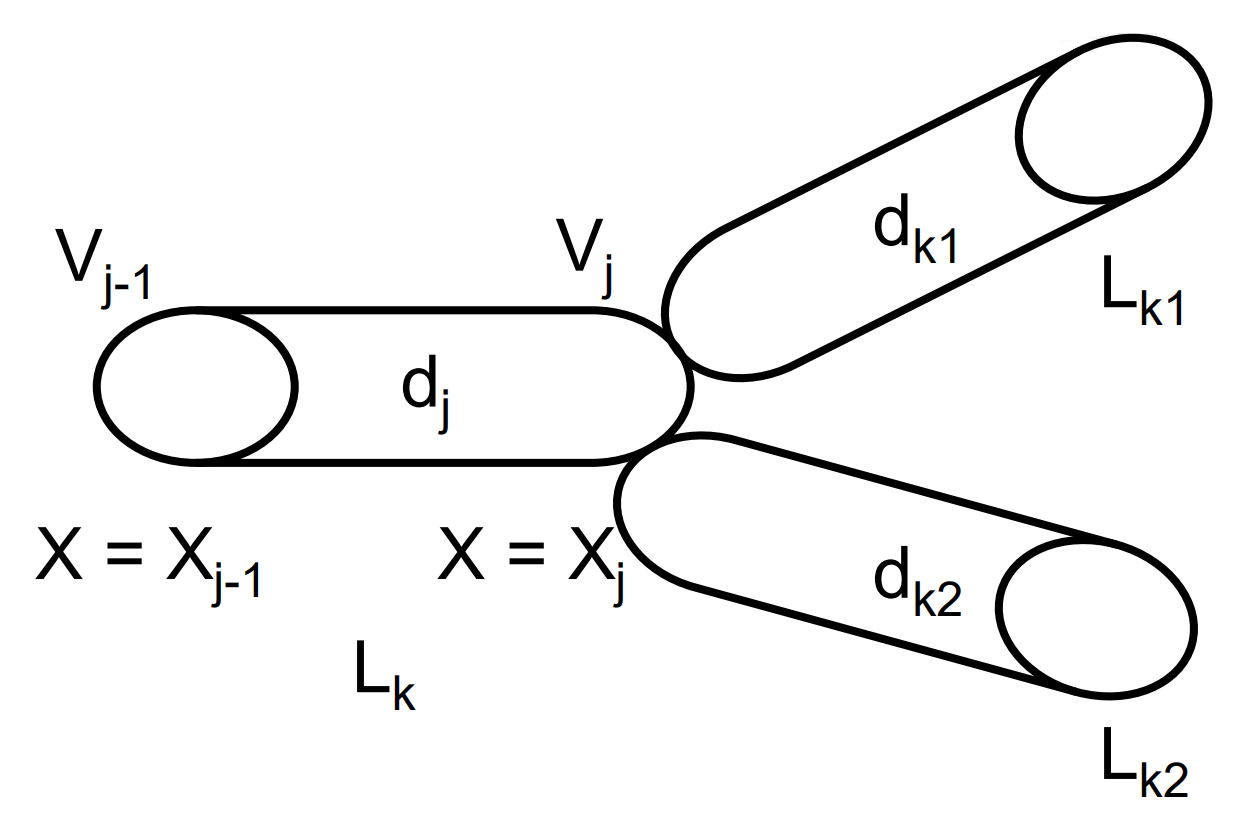
\includegraphics[scale=0.2]{03_6}
    \centering
\end{figure}
The Rall's model can be used with neurons matching three particularly strict criteria:
\begin{enumerate}
    \item The electrotonic lengths of all paths from soma to dendritic ends must be identical.
          \begin{equation*}
              L_{k}=L_{k1}=L_{k2}
          \end{equation*}
    \item The sum of the diameters of child branches at each branch point, raised to the power
          of \(\frac{3}{2}\) must equal the diameter of the parent branch, also raised to the power
          of \(\frac{3}{2}\).
          \begin{equation*}
              (d_{j})^{\frac{3}{2}}=(d_{k1})^{\frac{3}{2}}+(d_{k2})^{\frac{3}{2}}
          \end{equation*}
    \item The electrical properties should be constant and uniform as much as possible, in
          particular \(R_{m}\) and \(R_{i}\) must be spatially uniform within the branching structure.
          \begin{figure}[H]
              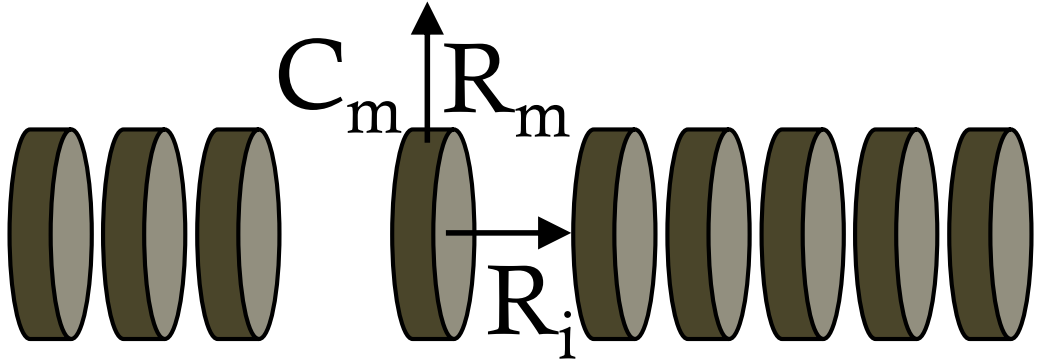
\includegraphics[scale=0.15]{03_7}
              \centering
          \end{figure}
\end{enumerate}
To sum up, the Rall's cable approach wants to substitute the whole dendritic tree with a single
cable having a constant diameter and the surface area distributed, with respect to the electrotonic
distance, similarly to the one of the original tree. Unfortunately, real neurons does not exhibit
morphological characteristics compliant with the Rall's criteria, therefore a less strict model
is to be introduced.
\paragraph{The Equivalent Cable}
This model was introduced to overcome the limitations of the Rall's cylinder, as a matter of
facts the idea is once again to model the whole dendritic tree as a single cable, but
the diameter is no longer assumed constant: it changes as a function of distance. This allows
a modelling much more precise in terms of electrical quantities, since they are strictly
related to the radius of the equivalent cable. A parameter \(\Delta{x}\) regulates the degree
of detail of the model, in particular it represents the length of a segment with constant
diameter of the overall cable. A very small \(\Delta{x}\) generates an extremely precise model,
but the computational cost increases as a consequence of the greater number of compartments.
\begin{figure}[H]
    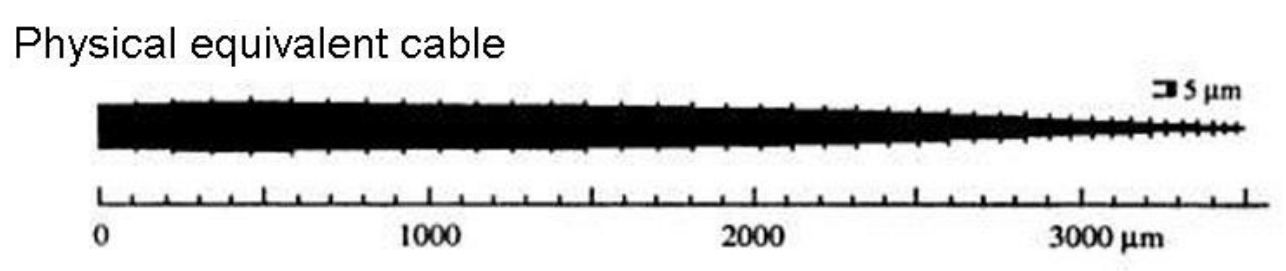
\includegraphics[scale=0.35]{03_8}
    \centering
\end{figure}
\paragraph{The Attenuation Cable}
The idea behind this approach is to disregard all the dendritic branches along which the
input signal attenuation overcomes a certain threshold: the assumption is that branches
exhibiting very fast decays are not important for the overall signal propagation.
\begin{figure}[H]
    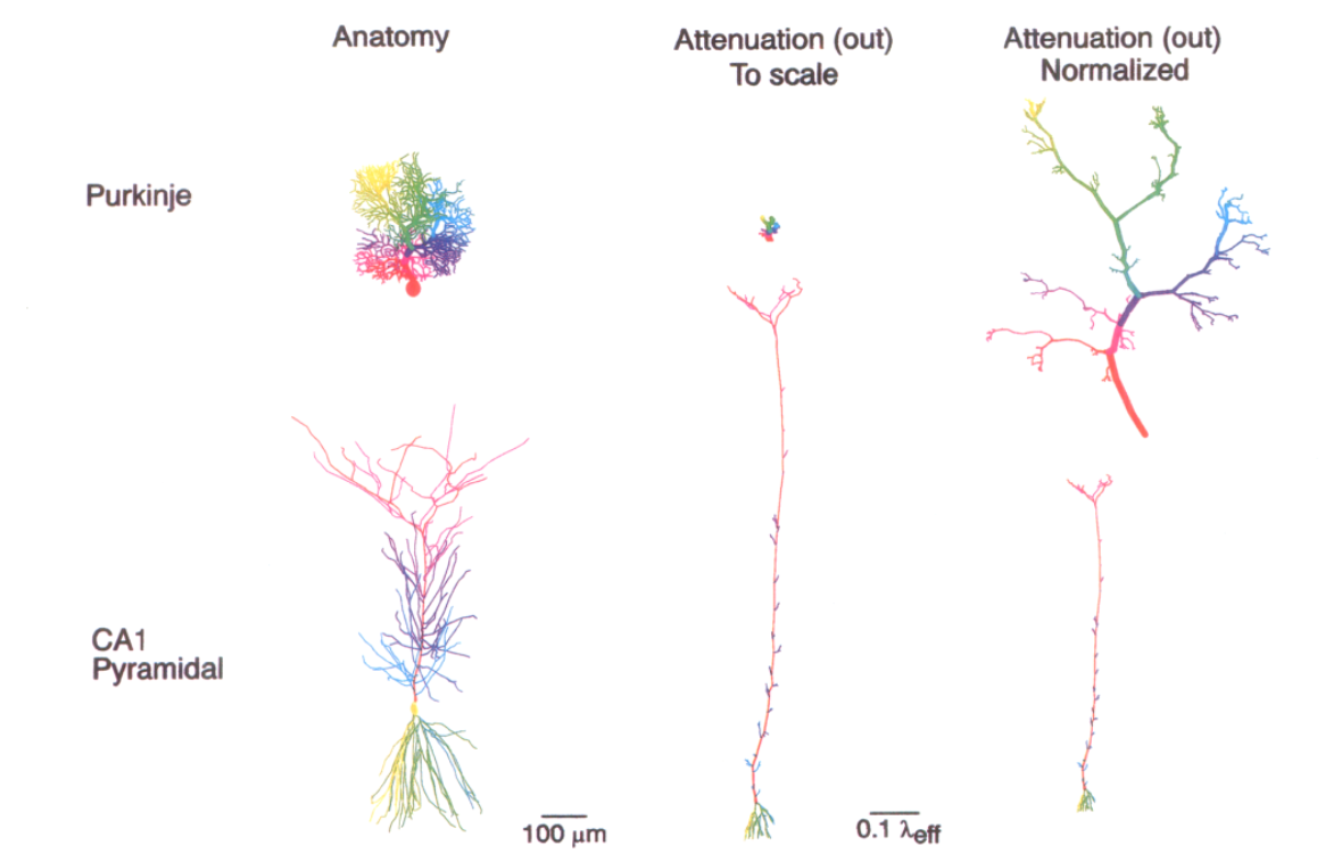
\includegraphics[scale=0.6]{03_9}
    \centering
\end{figure}
Note that the voltage attenuation is not an appropriate quantity to represent geometrically,
as it is not additive. To obtain the attenuation and delay of the membrane potential
for complex morphologies it is better to proceed as illustrated below.
\begin{figure}[H]
    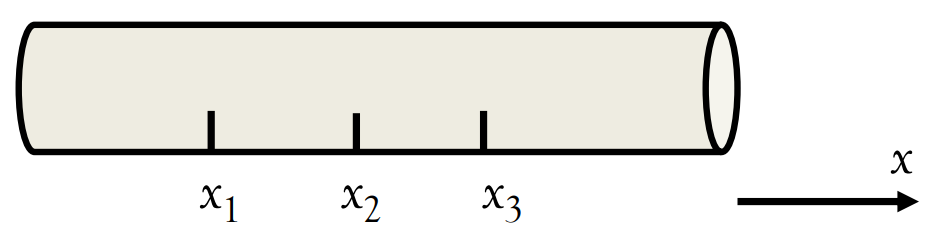
\includegraphics[scale=0.3]{03_10}
    \centering
\end{figure}
The voltage attenuation between \(x_{1}\) and \(x_{3}\) is:
\begin{equation*}
    \frac{V(x_{1})}{V(x_{3})}=\frac{V(x_{1})}{V(x_{2})}\cdot{\frac{V(x_{2})}{V(x_{3})}}
\end{equation*}
By applying the logarithm, an additive quantity is obtained, providing better information
about the signal propagation.
\begin{equation*}
    \ln{\biggl(\frac{V(x_{1})}{V(x_{3})}\biggr)}=
    \ln{\biggl(\frac{V(x_{1})}{V(x_{2})}\biggr)}+\ln{\biggl(\frac{V(x_{2})}{V(x_{3})}\biggr)}
\end{equation*}
Note that a similar approach considering signal propagation delay instead of signal
attenuation also exists.
\paragraph{The Pinsky-Rinzel 2-Comp Model}
This model is based on the fact that at least two compartments are required to properly mimic
complex patterns of electrophysiological activity. In particular, a compartment models the soma,
while another approximates the dendrites.
\begin{figure}[H]
    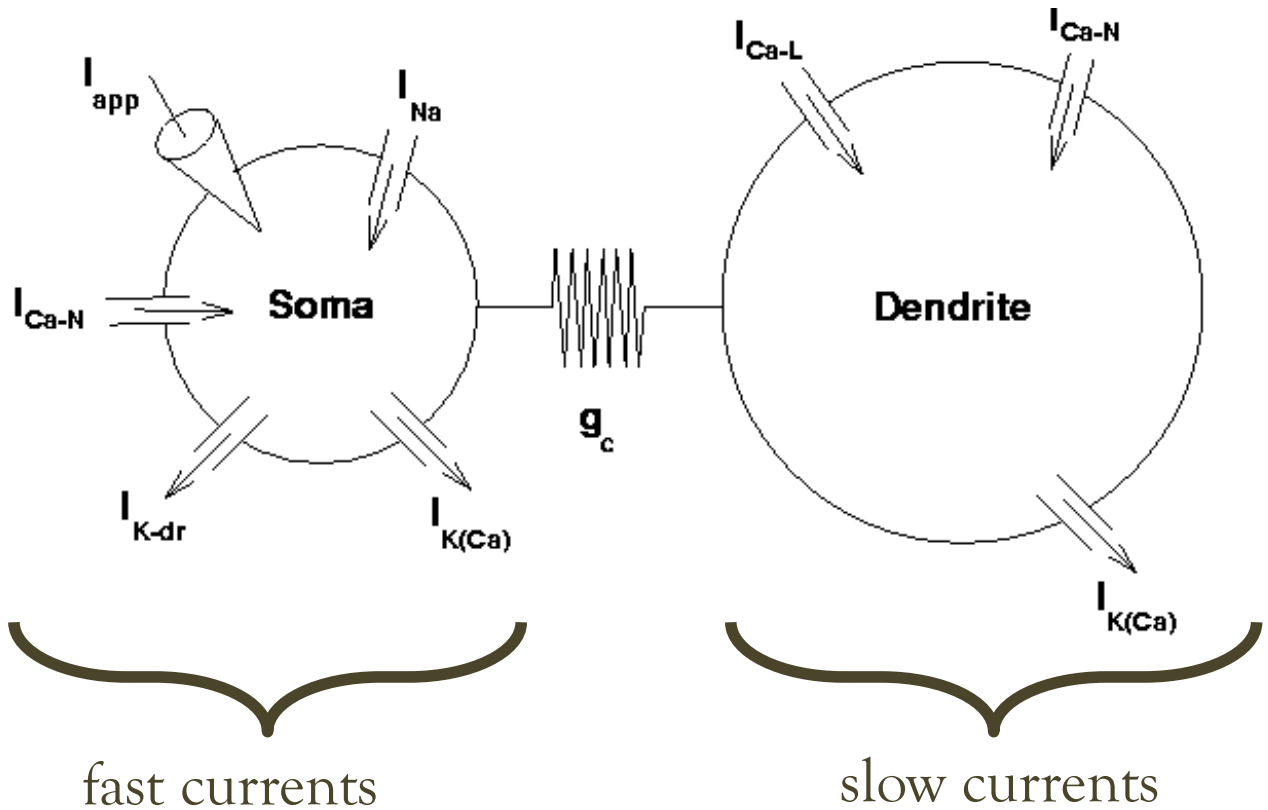
\includegraphics[scale=0.3]{03_11}
    \centering
\end{figure}
These two compartments are separated by a conductance \(g_{c}\) determining the coupling between
them, which instead regulates the kind of electrophysiological activity.
\begin{figure}[H]
    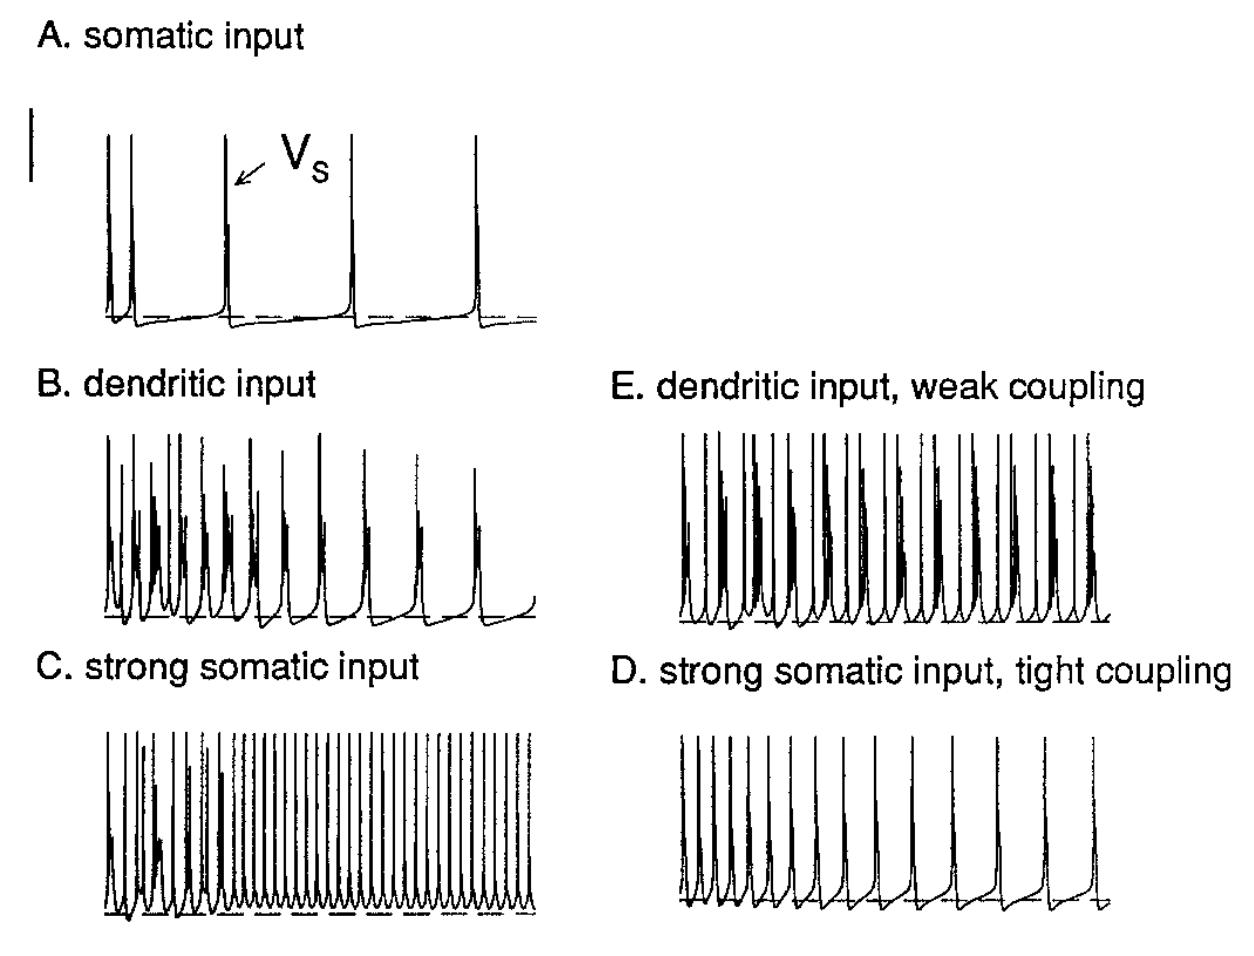
\includegraphics[scale=0.3]{03_12}
    \centering
\end{figure}

\subsection{Modelling Dendritic Spines and Synaptic Inputs}
Spines should definitely be taken into account when building the model of a neuron, they
characterize the surface of dendrites, moreover spines usually contain synapses.
\begin{figure}[H]
    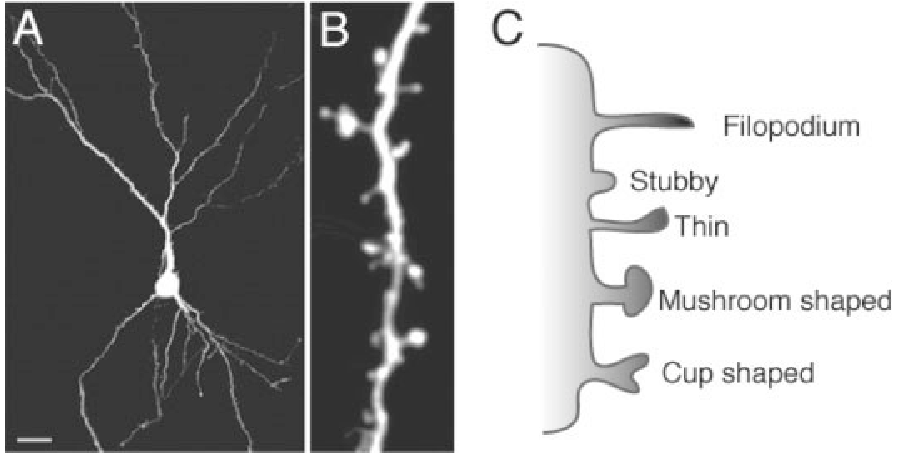
\includegraphics[scale=0.5]{03_13}
    \centering
\end{figure}
Note that several shapes are available when talking about spines, with different
geometrical properties and, as a consequence, different electrical properties.\\
When modelling spines, two distinct cases should be taken into account:
\begin{itemize}
    \item \textbf{Sipnes as \textit{passive} components}: the current flows \textit{from}
          the dendrite \textit{into} the spines.\\
          This means that spines are considered to be without synapses (no inputs). They are
          isopotential and the membrane area can be incorporated into the membrane of the parent dendrite.
          \begin{figure}[H]
              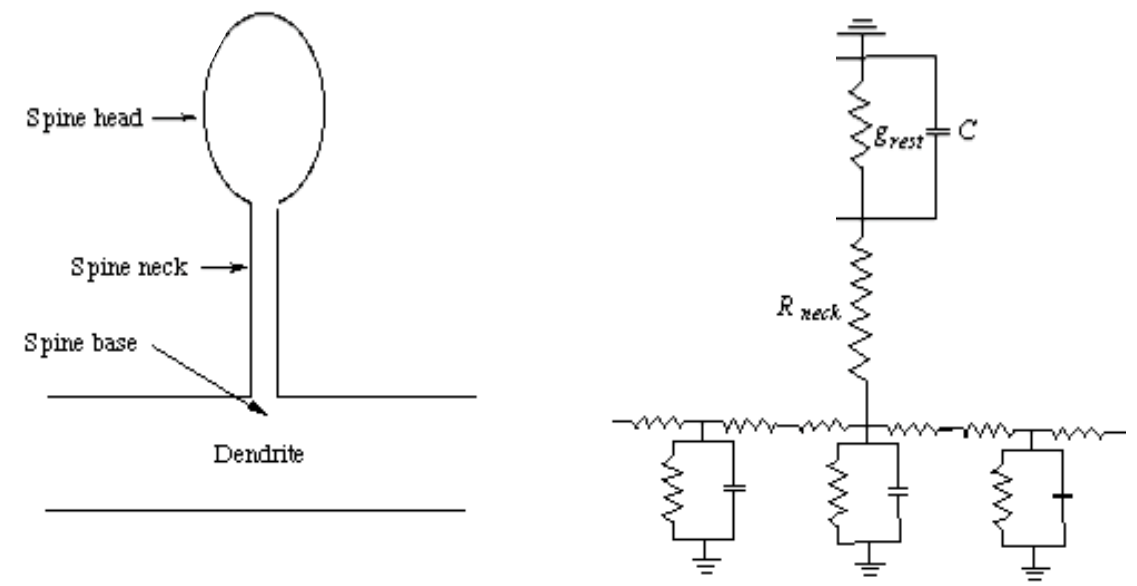
\includegraphics[scale=0.4]{03_14}
              \centering
          \end{figure}
          Both the physical dimensions and the specific membrane properties are affected by the presence
          of the spine:
          \begin{equation*}
              l'=l\cdot{F^{\frac{2}{3}}}
              \hspace{2.5cm}
              R_{m}'=\frac{R_{m}}{F}
          \end{equation*}
          \begin{equation*}
              d'=d\cdot{F^{\frac{2}{3}}}
              \hspace{2.5cm}
              C_{m}'=\frac{C_{m}}{F}
          \end{equation*}
          \begin{equation*}
              F=\frac{A_{dendrite}+A_{spine}}{A_{dendrite}}
          \end{equation*}
    \item \textbf{Sipnes as \textit{active} components}: the current is generated at the head membrane.\\
          In this case the spine contains a synapse, as an input current flows into it. The synaptic input
          can be modelled through a time-varying synaptic conductance.
          \begin{figure}[H]
              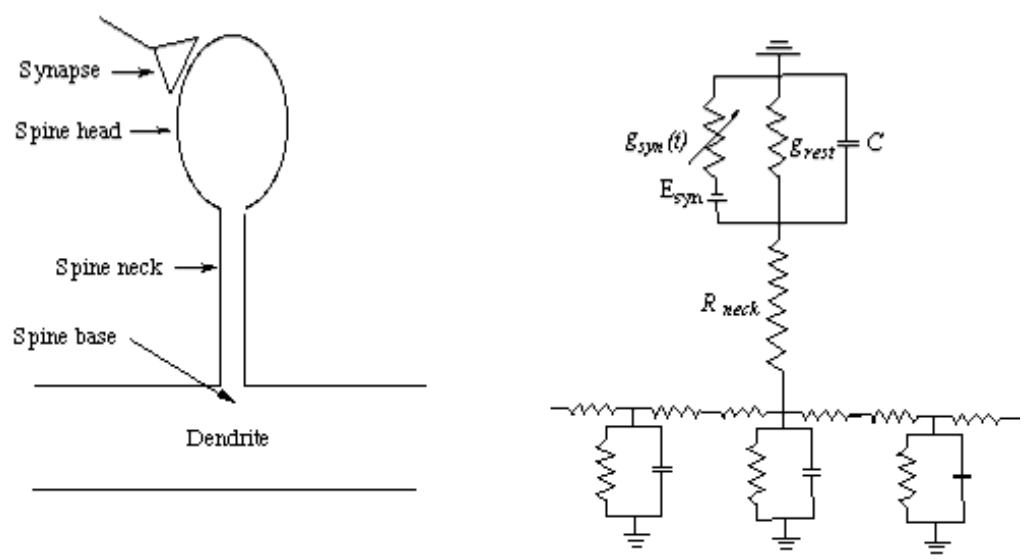
\includegraphics[scale=0.4]{03_15}
              \centering
          \end{figure}
          Here the factor \(F\) used in the
          other case can no longer be employed, as each spine exhibits its own kinetics.
\end{itemize}